% ================================================================================
%
% Copyright (c) 2009--2011, Nico Schlömer
% All rights reserved.
% 
% Redistribution and use in source and binary forms, with or without
% modification, are permitted provided that the following conditions are
% met:
% 
%     * Redistributions of source code must retain the above copyright
%       notice, this list of conditions and the following disclaimer.
%     * Redistributions in binary form must reproduce the above copyright
%       notice, this list of conditions and the following disclaimer in
%       the documentation and/or other materials provided with the distribution
% 
% THIS SOFTWARE IS PROVIDED BY THE COPYRIGHT HOLDERS AND CONTRIBUTORS "AS IS"
% AND ANY EXPRESS OR IMPLIED WARRANTIES, INCLUDING, BUT NOT LIMITED TO, THE
% IMPLIED WARRANTIES OF MERCHANTABILITY AND FITNESS FOR A PARTICULAR PURPOSE
% ARE DISCLAIMED. IN NO EVENT SHALL THE COPYRIGHT OWNER OR CONTRIBUTORS BE
% LIABLE FOR ANY DIRECT, INDIRECT, INCIDENTAL, SPECIAL, EXEMPLARY, OR
% CONSEQUENTIAL DAMAGES (INCLUDING, BUT NOT LIMITED TO, PROCUREMENT OF
% SUBSTITUTE GOODS OR SERVICES; LOSS OF USE, DATA, OR PROFITS; OR BUSINESS
% INTERRUPTION) HOWEVER CAUSED AND ON ANY THEORY OF LIABILITY, WHETHER IN
% CONTRACT, STRICT LIABILITY, OR TORT (INCLUDING NEGLIGENCE OR OTHERWISE)
% ARISING IN ANY WAY OUT OF THE USE OF THIS SOFTWARE, EVEN IF ADVISED OF THE
% POSSIBILITY OF SUCH DAMAGE.
%
% ================================================================================
\newpage
\section{Other tips \& tricks}

% \begin{listing}
% \begin{minted}[frame=single,framerule=2pt,color=\color{badred}]{matlab}
% % ===================================================
% % *** FUNCTION simpson
% % ***
% % *** Implements Simpson's rule for integrating
% % *** the sine function over [a,b] with granularity
% % *** h.
% % ***
% % ===================================================
% function int = simpson( a, b, h )
% 
%   x = a:h:b;
% 
%   int = 0;
%   n   = length(x);
%   mid = (x(1:n-1) + x(2:n)) / 2;
%   int = sum( h/6 * (    sin(x(1:n-1)) ...
%                     + 4*sin(mid     ) ...
%                     +   sin(x(2:n  )) ) );
% 
% end
% % ===================================================
% % *** END FUNCTION simpson
% % ===================================================
% \end{minted}
% \caption{Implementation of Simpson's rule for numerically integrating a function (here: \lstinline!sin!) between \lstinline!a! and \lstinline!b!. Note the usage of the vector notation to speed up the function. Also note that \lstinline!sin! is hardcoded into the routine, and needs to be changed each time we want to change the function. In case one is interested in calculating the integral of $f(x) = \exp(\sin(\frac{1}{x})) / \tan(\sqrt{1-x^4})$, this could get quite messy.}
% \label{listing:simpson1}
% \end{listing}


\begin{lstlisting}[
framerule=2pt,
float,
label={listing:simpson1},
caption={Implementation of Simpson's rule for numerically integrating a function (here: \lstinline!sin!) between \lstinline!a! and \lstinline!b!. Note the usage of the vector notation to speed up the function. Also note that \lstinline!sin! is hardcoded into the routine, and needs to be changed each time we want to change the function. In case one is interested in calculating the integral of $f(x) = \exp(\sin(\frac{1}{x})) / \tan(\sqrt{1-x^4})$, this could get quite messy.},
rulecolor=\color{badred}]
% ===================================================
% *** FUNCTION simpson
% ***
% *** Implements Simpson's rule for integrating
% *** the sine function over [a,b] with granularity
% *** h.
% ***
% ===================================================
function int = simpson( a, b, h )

  x = a:h:b;

  int = 0;
  n   = length(x);
  mid = (x(1:n-1) + x(2:n)) / 2;
  int = sum( h/6 * (    sin(x(1:n-1)) ...
                    + 4*sin(mid     ) ...
                    +   sin(x(2:n  )) ) );

end
% ===================================================
% *** END FUNCTION simpson
% ===================================================
\end{lstlisting}

\subsection{Functions as arguments -- \cleansymbol\cleansymbol\cleansymbol}

In numerical computation, there are set-ups which natively treat functions as the objects of interest, for example when numerically integrating them over a particular domain. For this example, imagine that you wrote a function that implements Simpson's integration rule (see listing \ref{listing:simpson1}), and you would like to apply it to a number of functions without having to alter your source code (for example, replacing \lstinline!sin()! by \lstinline!cos()!, \lstinline!exp()! or something else).

A clean way to deal with this in \matlab{} is using \emph{function handles}. This may sound fancy, and describes nothing else then the capability of treating functions (such as \lstinline!sin()!) as arguments to other functions (such as \lstinline!simpson()!). The function call itself is written as easy as

\begin{lstlisting}[
float,
caption={Simpson's rule with function handles. Note that the syntax for function arguments is no different from that of ordinary ones.},
label={listing:simpson2},
framerule=2pt,
rulecolor=\color{goodgreen}]
% ===================================================
% *** FUNCTION simpson
% ***
% *** Implements Simpson's rule for integrating
% *** a function f over [a,b] with granularity h.
% ***
% ===================================================
function int = simpson( f, a, b, h )

  x   = a:h:b;
  mid = (x(1:n-1) + x(2:n)) / 2;

  n   = length(x);

  int = sum( h/6 * (    f(x(1:n-1)) ...
                    + 4*f(mid     ) ...
                    +   f(x(2:n  )) ) );

end 
% ===================================================
% *** END FUNCTION simpson
% ===================================================
\end{lstlisting}

\hfill
\begin{minipage}[t]{.90\textwidth}
\begin{lstlisting}[framerule=1pt,rulecolor=\color{goodgreen}]
a = 0;
b = pi/2;
h = 1e-2;
int_sin = simpson( @sin, a, b, h );
int_cos = simpson( @cos, a, b, h );
int_f   = simpson( @f  , a, b, h );
\end{lstlisting}
\end{minipage}
\hfill

where the function name need to be prepended by the `\lstinline!@!'-character.

The function \lstinline!f()! can be any function that you defined yourself and which is callable as \lstinline!f(x)! with \lstinline!x! being a vector of $x$ values (like it is used in \lstinline!simpson()!, listing \ref{listing:simpson2}).



\subsection{Implicit matrix--vector products -- \cleansymbol}

In numerical analysis, almost all methods for solving linear equation systems \emph{quickly} are iterative methods, that is, methods which define how to iteratively approach a solution in small steps (starting with some initial guess) rather then directly solving them in one big step (such as Gau{\ss}ian elimination). Two of the most prominent iterative methods are CG and GMRES.

In particular, those methods \emph{do not require the explicit availability of the matrix} as in each step of the iteration they merely form a matrix-vector product with $A$ (or variations of it). Hence, they technically only need a function to tell them how to carry out a matrix-vector multiplication. In some cases, providing such a function may be easier than explicitly constructing the matrix itself, as the latter usually requires one to pay close attention to indices (which can get extremely messy).

Beyond that, there may also a mild advantage in memory consumption as the indices of the matrix do no longer need to sit in memory, but can be hardcoded into the matrix-vector-multiplication function itself. Considering the fact that we are mostly working with sparse matrices however, this might not be quite important.

The example below illustrates the typical benefits and backdraws of the approach.

\begin{lstlisting}[
float,
framerule=1pt,
caption={Function that implements matrix--vector multiplication with $1/h^2 \times \diag(-1,2,-1)$. Note that the function consumes (almost) no more memory then \lstinline!u! already required.},
label={listing:Amultiply}
]
% ===================================================
% *** FUNCTION A_multiply
% ***
% *** Implements matrix--vector multiplication with 
% *** diag[-1,2,-1]/h^2  .
% ***
% ===================================================
function out = A_multiply( u )

  n   = length( u );
  u   = [0; u; 0];

  out = -u(1:n) + 2*u(2:n+1) - u(3:n+2);
  out = out * (n+1)^2;

end 
% ===================================================
% *** END FUNCTION A_multiply
% ===================================================
\end{lstlisting}


\hfill
\begin{minipage}[t]{.45\textwidth}
\begin{lstlisting}[framerule=1pt]
n = 1e3;
k = 500;







u = ones(n,1);
for i=1:k
    u = A_multiply( u );
end
\end{lstlisting}
Computing $u = A^ku_0$ with the function \lstinline!A_multiply! (listing \ref{listing:Amultiply}). The memory consumption of this routine is (almost) no greater than storing $n$ real numbers. Execution time: \extime{21}.
\end{minipage}
\hfill
\begin{minipage}[t]{.45\textwidth}
\begin{lstlisting}[framerule=1pt]
n = 1e3;
k = 500;

e = ones(n,1);
A = spdiags([-e,2*e,-e],...
            [-1,  0,-1],...
             n, n );
A = A * (n+1)^2;

u = ones(n,1);
for i=1:k
    u = A*u;
end
\end{lstlisting}
Computing $u = A^ku_0$ with a regular sparse format matrix \lstinline!A!, with the need to store it in memory. Execution time: \extime{7}.
\end{minipage}
\hfill

All in all, these considerations shall not lead you to rewrite all you matrix-vector multiplcations as function calls. Mind, however, that there are sitatuations where one would \emph{never} use matrices in their explicit form, although mathematically written down like that:

\begin{example}[Multigrid]
In geometric multigrid methods, a domain is discretized with a certain parameter $h$ (``grid width'') and the operator $A_h$ written down for that discretization (see the examples above, where $A_h=h^{-2}\diag(-1,2,1)$ is really the discretization of the $\Delta$-operator in one dimension). In a second step, another, somewhat coarser grid is considered with $H=2h$, for example. The operator $A_H$ on the coarser grid is written down as
\[
A_H = I_h^H A_h I_H^h,
\]
where the $I_*^*$ operators define the transition from the coarse to the fine grid, or the other way around. When applying it to a vector on the coarse grid $u_H$ ($A_Hu_H =I_h^H A_h I_H^h u_H$), the above definition reads:
\begin{enumerate}
\item $I_H^h u_H$: Map $u_H$ to the fine grid.
\item $A_h\cdot$: Apply the fine grid operator to the transformation.
\item $I_h^H\cdot$: Transform the result back to the coarse grid.
\end{enumerate}
How the transformations are executed needs to be defined. One could, for example, demand that $I_H^h$ maps all points that are part of the fine grid \emph{and} the coarse grid to itself; all points on the fine grid, that lie right in between two coarse variables get half of the value of each of the two (see figure \ref{subfig:coarse-fine}).

\begin{figure}
\hfill
\subfloat[][]{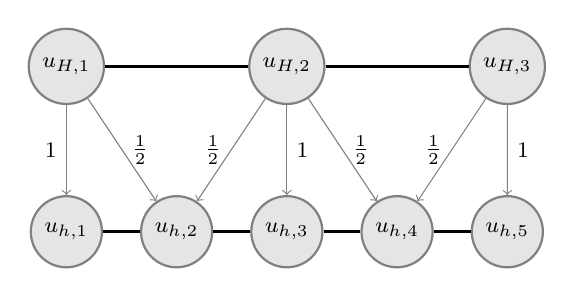
\begin{tikzpicture}[node/.style={circle,draw=black!50,fill=black!10,thick,font=\footnotesize},scale=0.7,
arrownote/.style={black,font=\footnotesize}]


\node (u1) at (0,3) [node] {$u_{H,1}$};
\node (u2) at (4,3) [node] {$u_{H,2}$};
\node (u3) at (8,3) [node] {$u_{H,3}$};


\node (u5) at (0,0) [node] {$u_{h,1}$};
\node (u6) at (2,0) [node] {$u_{h,2}$};
\node (u7) at (4,0) [node] {$u_{h,3}$};
\node (u8) at (6,0) [node] {$u_{h,4}$};
\node (u9) at (8,0) [node] {$u_{h,5}$};

\draw [very thick] (u1) -- (u2) --(u3);
\draw [very thick] (u5) --(u6) --(u7) --(u8) --(u9);

\draw [->,black!50] (u1) to node [arrownote,left] {$1$}  (u5) ;
\draw [->,black!50] (u1) to node [arrownote,right] {$\frac{1}{2}$} (u6) ;

\draw [->,black!50] (u2) to node [arrownote,left] {$\frac{1}{2}$} (u6) ;
\draw [->,black!50] (u2) to node [arrownote,right] {$1$} (u7) ;
\draw [->,black!50] (u2) to node [arrownote,right] {$\frac{1}{2}$} (u8) ;

\draw [->,black!50] (u3) to node [arrownote,left] {$\frac{1}{2}$} (u8) ;
\draw [->,black!50] (u3) to node [arrownote,right] {$1$} (u9) ;

\end{tikzpicture}\label{subfig:coarse-fine}}
\hfill
\subfloat[][]{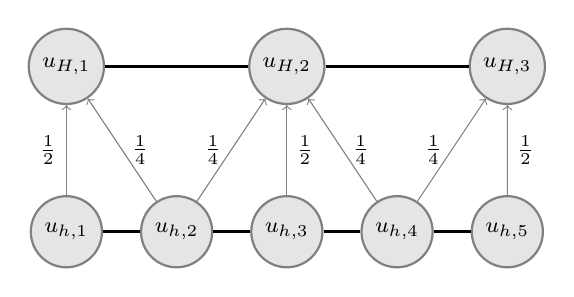
\begin{tikzpicture}[
node/.style={circle,draw=black!50,fill=black!10,thick,font=\footnotesize},scale=0.7,
arrownote/.style={black,font=\footnotesize}]


\node (u1) at (0,3) [node] {$u_{H,1}$};
\node (u2) at (4,3) [node] {$u_{H,2}$};
\node (u3) at (8,3) [node] {$u_{H,3}$};


\node (u5) at (0,0) [node] {$u_{h,1}$};
\node (u6) at (2,0) [node] {$u_{h,2}$};
\node (u7) at (4,0) [node] {$u_{h,3}$};
\node (u8) at (6,0) [node] {$u_{h,4}$};
\node (u9) at (8,0) [node] {$u_{h,5}$};

\draw [very thick] (u1) -- (u2) --(u3);blue
\draw [very thick] (u5) --(u6) --(u7) --(u8) --(u9);

\draw [->,black!50] (u5) to node [arrownote,left] {$\frac{1}{2}$}  (u1) ;
\draw [->,black!50] (u6) to node [arrownote,right] {$\frac{1}{4}$} (u1) ;

\draw [->,black!50] (u6) to node [arrownote,left] {$\frac{1}{4}$} (u2) ;
\draw [->,black!50] (u7) to node [arrownote,right] {$\frac{1}{2}$} (u2) ;
\draw [->,black!50] (u8) to node [arrownote,right] {$\frac{1}{4}$} (u2) ;

\draw [->,black!50] (u8) to node [arrownote,left] {$\frac{1}{4}$} (u3) ;
\draw [->,black!50] (u9) to node [arrownote,right] {$\frac{1}{2}$} (u3) ;

\end{tikzpicture}\label{subfig:fine-coarse}}
\hfill

\caption{\subref{subfig:coarse-fine} Possible transformation rule when translating values from the coarse to the fine grid. See listing \ref{listing:IHh}. \subref{subfig:fine-coarse} Mapping back from the fine to coarse.}
\end{figure}


\begin{lstlisting}[
float,
framerule=1pt,
caption={Function that implements the operator $I_H^h$ from the example (see figure \ref{subfig:coarse-fine}). Writing down the structure of the corresponding matrix would be somewhat complicated, and even more so when moving to two- or three-dimensional grids. Note also how matrix notation has been exploited.},
label={listing:IHh}
]
% ===========================================================
% *** FUNCTION coarse2fine
% ***
% *** Transforms values from a coarse grid to a fine grid.
% ***
% ===========================================================
function uFine = coarse2fine( uCoarse )

  N = length(uCoarse);
  n = 2*N - 1;

  uFine(1:2:n) = uCoarse;

  midValues    = 0.5 * ( uCoarse(1:N-1) + uCoarse(2:N) );
  uFine(2:2:n) = midValues;

end
% ===========================================================
% *** END FUNCTION coarse2fine
% ===========================================================
\end{lstlisting}


In the analysis of the method, $I_H^h$ and $I_h^H$ will always be treated as matrices, but when implementing, one would \emph{certainly not} try to figure out the structure of the matrix. It is a lot simpler to implement a function that executes the rule suggested above, for example.
\end{example}


% In het verdere verloop van de cursus zal het duidelijk worden dat iteratieve methoden de oplossing vinden zonder een expliciete
% uitdrukking voor de matrix $A$.  De oplossing kan gevonden worden met matrix vector producten $A v$ waar de matrix toegepast wordt op een
% gegeven vector $v$.  Inderdaad, de Richardson iteratie $x_{k+1} = (I - A) x_k + b$ kan uitgevoerd worden als we over een routine \texttt{matvec}
% beschikken die voor een gegeven input vector $v$ het resultaat $A v$ terug geeft.  Om $x_{k+1}$ uit te rekenen, tellen we bij het matrix-vector product $-A x_k$ de vector $x_k + b$ op.
% 
% In de verdere hoofdstukken van de cursus wordt het duidelijk dat ook Krylov methoden slechts gebruik maken van de matrix $A$ toegepast op een vector $v$.
% 
% 
% 
% Daarom geven we in hier aandacht aan de effici\"ente implementatie van de matrix-vector producten.
% 
% \section{Matrix-Vector routines}
% Onderstel dat $A$ een centrale differentie voorstelling is van de eerste afgeleide operator
% \begin{equation}
% 	u'(x_i) = \frac{u(x_{i+1})-u(x_{i-1})}{2 \Delta x}
% \end{equation}
% of in matrix notatie
% \begin{equation}
% 	\begin{pmatrix}
% 		 u'(x_1)\\
% 		 u'(x_2)\\
% 		\vdots \\
%                  u'(x_N)
% 	\end{pmatrix}
% 	 =  \frac{1}{2 h}\begin{pmatrix}
% 	  0 &  1      &        &   \\
% 	 -1 &  \ddots & \ddots &   \\
%     	    &  \ddots & \ddots & 1 \\
% 	    &         &  -1    & 0
% 	\end{pmatrix}
% 	\begin{pmatrix}
% 		 u(x_1)\\
% 		 u(x_2)\\
% 		\vdots \\
%                           u(x_N)
% 	\end{pmatrix}
% \end{equation}
% Het resultaat van deze matrix-vector vermenigvuldiging kan op een
% eenvoudiger manier verkregen worden door met de vector $u(x_i)$
% met $i \in \{1,\dots, N\}$ te werken.   Dit vermijdt ook dat we het matrix-vector product van hierboven expliciet uitrekenen omdat veel van deze vermenigvuldigingen met nul zijn.
% 
% In figuur \ref{uprime} tonen we hoe we door de vector $(u(x_0),
% u(x_1),\dots, u(x_N), u(x_{N+1}))$ naar links en rechts te
% verschuiven en samen te tellen, de eerste afgeleide kunnen uitrekenen.
% \begin{figure}[p]
% \centering
% % \includegraphics[width=12cm,height=8cm]{figures/matvec_uprime}
% % \includegraphics[width=12cm,height=8cm]{figures/matvec_uprime2}
% 	\caption{Om de eerste afgeleide, $u'$, in het punt $x_i$
% 	uit te rekenen met behulp van eindige differenties, tellen we $u(x_{i+1})$, voorgesteld met $\circ$, en $-u(x_{i-1})$, voorgesteld met $\times$, samen.  Dit kan gebeuren in een vectoroperatie door eerst $u$ (voorgesteld met $+$) \'e\'en roosterpunt naar links op te schuiven en daarbij de verschijving van $-u$ naar rechts op te  tellen.   Merk op dat wanneer we $u$ opschuiven, we in het laatste roosterpunt rekening moeten houden met  de randvoorwaarden. In dit voorbeeld zijn er Dirichlet randvoorwaarden $u(0)=0$ en $u(1)=0$.  Resultaat is dat de tweede afgeleide als een vectoroperatie geschreven kan worden.  \label{uprime}}
% 
% \end{figure}
% \begin{table}
% \begin{lstlisting}
% function Av = matvec(v)
% % Toepassing van de eindige differentie matrix op een vector u.
% % Vector uitbreiden met twee ghostcellen waarin we
% % de Dirichlet randvoorwaarden invullen.
% n = length(v);
% h = 1/(n+1);
% v = [0,v,0];
% Av = (v(3:end)-v(1:end-2))/(2*h)
% \end{lstlisting}
% \caption{$v$ is een vector van lengte $n$}
% \end{table}
% Op een analoge manier kunnen we matvec routines maken om de tweede afgeleide uit te rekenen.
% 
% \subsubsection*{Matvec voor tweede afgeleiden}
% Hier zijn enkele effici\"entere methoden.  Stel dat je het product $A v$
% moet uitrekenen waarbij $A$ een eindige differentie voorstelling  is van de
% tweede afgeleide operator en de vector $v_i = v(x_i)$ bevat de functie waarden in de rooster punten $x_i$.
% 
% We kunnen $\sum_{j=1}^N A_{ij} v_j = v_{i+1} -2v_i + v_{i-1}$ nu eenvoudig uitrekenen met \texttt{Matlab} met behulp van de volgende \texttt{matvec(v)} routine
% \begin{lstlisting}
% function Av = matvec(v)
% n = length(v);
% h = 1/(n+1);
% % Voeg zowel links als rechts een ghostcell toe.
% v = [0,v,0];
% % Bereken de tweede afgeleide.
% Av = (v(1:end-2)-2*v(2:end-1)+v(3:end))/h^2;
% \end{lstlisting}
% waarbij we aan de vector $v$ twee \textit{ghostcellen} toevoegen met de nul randvoorwaarden.  Hierdoor kan de tweede afgeleide voor de ganse vector in \'e\'en keer uitgerekend worden als een som van slices van vectoren.
% 
% In twee dimensies is de tweede afgeleide in de eindige differentie representatie
% \begin{equation}
% f''_{ij} =   \left( -4 f_{ij} + f_{i+1,j}  + f_{i-1,j} + f_{i,j+1} + f_{i,j-1} \right)/h^2.
% \end{equation}
% dit wordt dan
% \begin{lstlisting}
% function Av = matvec2D(v)
% n = sqrt(length(v));
% h = 1/(n+1);
% % Construeer een (n+2) bij (n+2) matrix.
% AV = zeros(n+2);
% % Transformeer de vector naar een matrix.
% AV(2:end-1,2:end-1) = reshape(v, n, n);
% % Bereken de tweede afgeleide.
% AV(2:end-1,2:end-1) = ( -4*AV(2:end-1,2:end-1)  ...
%                          + AV(1:end-2,2:end-1)  ...
%                          + AV(3:end,2:end-1)    ...
%                          + AV(2:end-1,1:end-2)  ...
%                          + AV(2:end-1,3:end)        ) /(h*h)
% % Transformeer terug naar een vector.
% Av = reshape(AV(2:end-1,2:end-1), n*n,1)
% \end{lstlisting}
% 
% Het probleem is nu dat de meeste iteratieve methoden die we besproken
% hebben ergens in de code een matrix-vector $Ax$ product moeten
% uitvoeren. Om flexibele programma's te schrijven, geven we dan als
% argument de \texttt{matvec} procedure mee in plaats van de matrix $A$.  Bijvoorbeeld {\tt
% mycg(A,b)} wordt nu opgeroepen als \texttt{mycg(matvec,b)}, waar {\tt
% matvec} je eigen gedefinieerde matrix-vector product routine is.
% 
% Om hiervan gebruik te kunnen maken, moet je de \texttt{matvec} functie
% als een \textit{function handle} defini\"eren. Als je bv. reeds een
% matrix $A$ hebt gedefinieerd, kan je met \texttt{matvec = @(x) A*x} een
% matvec routine maken die je met \texttt{mycg(matvec,b)} kan meegeven.  In de code vervang je dan \texttt{A*x} door \texttt{matvec(x)}.
% 
% Of als je reeds een \texttt{matvec\_functie\_met\_parameter(x,lambda)} hebt geprogrammeerd waarin een parameter $\lambda$ voorkomt, kan je een matvec defini\"eren \texttt{matvec = @(x)  matvec\_functie\_met\_parameter(x,12.5)}
% waarin de parameter $\lambda$ gelijk is gesteld aan 12.5.
% 
% {\bf Opdracht} Zoek eens op in de handleiding van Matlab hoe je omgaat met een \textit{function handle}.
